\section{Results of the exact computations}\label{sec:results}

Every number in this section is read from the saved certificates of EXP-001 and EXP-002 and from the output of the independent recomputation, by the script \texttt{make\_tables.py} that writes the tables and figure fragments of the paper and asserts each consistency condition the text uses.
All counts are exact integers; no sampling is involved, so no confidence interval is reported.

\subsection{The 75 shell constructions}\label{sec:res-shell}

The grid contains every $k=3,\ldots,12$ and every $a=2,\ldots,k+1$, which is $\sum_{k=3}^{12}k=\NGraphs$ graphs, of orders $\NOrderMin$ to $\NOrderMax$ and sizes $\NEdgeMin$ to $\NEdgeMax$.
Table~\ref{tab:shell75} lists each one.
All \NGraphs\ graphs have $\e(G)=\lceil kn/2\rceil$ and the predicted degree pattern, all have independence number $a$ and connectivity exactly $k$ in the independent recomputation, and each of the first-implementation checks (degree, edge count, recursive independence number, vertex-split flow connectivity) passed.
For the \NDirect\ graphs of order at most 16 the direct subset enumeration of $\alpha$ and the exhaustive vertex-deletion test of $\kappa$ agree with these checks.

\needspace{10\baselineskip}
{\scriptsize\setlength{\tabcolsep}{3.4pt}
\begin{longtable}{rrrlrrrrrrrl}
\caption{The 75 constructions of the shell grid, one row per $(k,a)$ with $n=a+k+1$. Construction: the residual used (cycle: complement of $C_n$; Harary: cycle power with a complement matching; matching: perfect matching on $k+1$ vertices; path: $P_{k+1}$; crown: $K_{a,a}$ minus a perfect matching). Columns $\kappa(G)$, $\alpha(G)$ and $\kappa(G-e)$ are recomputed with NetworkX 3.4.1 from the saved edge lists, where $e$ is the edge deleted in the damaged-edge control; $g=k-a$ and $\kappa(H)$ are the residual requirement and the recomputed connectivity of the augmented residual graph in the Harary rows; the last column marks the 45 constructions of order at most 16 also checked by direct subset and vertex-deletion enumeration.}\label{tab:shell75}\\
\toprule
$k$ & $a$ & $n$ & Construction & $\e(G)$ & $\varepsilon$ & $\kappa(G)$ & $\alpha(G)$ & $\kappa(G-e)$ & $g$ & $\kappa(H)$ & Direct\\
\midrule
\endfirsthead
\toprule
$k$ & $a$ & $n$ & Construction & $\e(G)$ & $\varepsilon$ & $\kappa(G)$ & $\alpha(G)$ & $\kappa(G-e)$ & $g$ & $\kappa(H)$ & Direct\\
\midrule
\endhead
\bottomrule
\endfoot
3 & 2 & 6 & cycle & 9 & 0 & 3 & 2 & 2 & -- & -- & yes\\
3 & 3 & 7 & matching & 11 & 1 & 3 & 3 & 2 & -- & -- & yes\\
3 & 4 & 8 & crown & 12 & 0 & 3 & 4 & 2 & -- & -- & yes\\
4 & 2 & 7 & cycle & 14 & 0 & 4 & 2 & 3 & -- & -- & yes\\
4 & 3 & 8 & path & 16 & 0 & 4 & 3 & 3 & -- & -- & yes\\
4 & 4 & 9 & matching & 18 & 0 & 4 & 4 & 3 & -- & -- & yes\\
4 & 5 & 10 & crown & 20 & 0 & 4 & 5 & 3 & -- & -- & yes\\
5 & 2 & 8 & cycle & 20 & 0 & 5 & 2 & 4 & -- & -- & yes\\
5 & 3 & 9 & Harary & 23 & 1 & 5 & 3 & 4 & 2 & 2 & yes\\
5 & 4 & 10 & path & 25 & 0 & 5 & 4 & 4 & -- & -- & yes\\
5 & 5 & 11 & matching & 28 & 1 & 5 & 5 & 4 & -- & -- & yes\\
5 & 6 & 12 & crown & 30 & 0 & 5 & 6 & 4 & -- & -- & yes\\
6 & 2 & 9 & cycle & 27 & 0 & 6 & 2 & 5 & -- & -- & yes\\
6 & 3 & 10 & Harary & 30 & 0 & 6 & 3 & 5 & 3 & 3 & yes\\
6 & 4 & 11 & Harary & 33 & 0 & 6 & 4 & 5 & 2 & 2 & yes\\
6 & 5 & 12 & path & 36 & 0 & 6 & 5 & 5 & -- & -- & yes\\
6 & 6 & 13 & matching & 39 & 0 & 6 & 6 & 5 & -- & -- & yes\\
6 & 7 & 14 & crown & 42 & 0 & 6 & 7 & 5 & -- & -- & yes\\
7 & 2 & 10 & cycle & 35 & 0 & 7 & 2 & 6 & -- & -- & yes\\
7 & 3 & 11 & Harary & 39 & 1 & 7 & 3 & 6 & 4 & 4 & yes\\
7 & 4 & 12 & Harary & 42 & 0 & 7 & 4 & 6 & 3 & 3 & yes\\
7 & 5 & 13 & Harary & 46 & 1 & 7 & 5 & 6 & 2 & 2 & yes\\
7 & 6 & 14 & path & 49 & 0 & 7 & 6 & 6 & -- & -- & yes\\
7 & 7 & 15 & matching & 53 & 1 & 7 & 7 & 6 & -- & -- & yes\\
7 & 8 & 16 & crown & 56 & 0 & 7 & 8 & 6 & -- & -- & yes\\
8 & 2 & 11 & cycle & 44 & 0 & 8 & 2 & 7 & -- & -- & yes\\
8 & 3 & 12 & Harary & 48 & 0 & 8 & 3 & 7 & 5 & 5 & yes\\
8 & 4 & 13 & Harary & 52 & 0 & 8 & 4 & 7 & 4 & 4 & yes\\
8 & 5 & 14 & Harary & 56 & 0 & 8 & 5 & 7 & 3 & 3 & yes\\
8 & 6 & 15 & Harary & 60 & 0 & 8 & 6 & 7 & 2 & 2 & yes\\
8 & 7 & 16 & path & 64 & 0 & 8 & 7 & 7 & -- & -- & yes\\
8 & 8 & 17 & matching & 68 & 0 & 8 & 8 & 7 & -- & -- & no\\
8 & 9 & 18 & crown & 72 & 0 & 8 & 9 & 7 & -- & -- & no\\
9 & 2 & 12 & cycle & 54 & 0 & 9 & 2 & 8 & -- & -- & yes\\
9 & 3 & 13 & Harary & 59 & 1 & 9 & 3 & 8 & 6 & 6 & yes\\
9 & 4 & 14 & Harary & 63 & 0 & 9 & 4 & 8 & 5 & 5 & yes\\
9 & 5 & 15 & Harary & 68 & 1 & 9 & 5 & 8 & 4 & 4 & yes\\
9 & 6 & 16 & Harary & 72 & 0 & 9 & 6 & 8 & 3 & 3 & yes\\
9 & 7 & 17 & Harary & 77 & 1 & 9 & 7 & 8 & 2 & 2 & no\\
9 & 8 & 18 & path & 81 & 0 & 9 & 8 & 8 & -- & -- & no\\
9 & 9 & 19 & matching & 86 & 1 & 9 & 9 & 8 & -- & -- & no\\
9 & 10 & 20 & crown & 90 & 0 & 9 & 10 & 8 & -- & -- & no\\
10 & 2 & 13 & cycle & 65 & 0 & 10 & 2 & 9 & -- & -- & yes\\
10 & 3 & 14 & Harary & 70 & 0 & 10 & 3 & 9 & 7 & 7 & yes\\
10 & 4 & 15 & Harary & 75 & 0 & 10 & 4 & 9 & 6 & 6 & yes\\
10 & 5 & 16 & Harary & 80 & 0 & 10 & 5 & 9 & 5 & 5 & yes\\
10 & 6 & 17 & Harary & 85 & 0 & 10 & 6 & 9 & 4 & 4 & no\\
10 & 7 & 18 & Harary & 90 & 0 & 10 & 7 & 9 & 3 & 3 & no\\
10 & 8 & 19 & Harary & 95 & 0 & 10 & 8 & 9 & 2 & 2 & no\\
10 & 9 & 20 & path & 100 & 0 & 10 & 9 & 9 & -- & -- & no\\
10 & 10 & 21 & matching & 105 & 0 & 10 & 10 & 9 & -- & -- & no\\
10 & 11 & 22 & crown & 110 & 0 & 10 & 11 & 9 & -- & -- & no\\
11 & 2 & 14 & cycle & 77 & 0 & 11 & 2 & 10 & -- & -- & yes\\
11 & 3 & 15 & Harary & 83 & 1 & 11 & 3 & 10 & 8 & 8 & yes\\
11 & 4 & 16 & Harary & 88 & 0 & 11 & 4 & 10 & 7 & 7 & yes\\
11 & 5 & 17 & Harary & 94 & 1 & 11 & 5 & 10 & 6 & 6 & no\\
11 & 6 & 18 & Harary & 99 & 0 & 11 & 6 & 10 & 5 & 5 & no\\
11 & 7 & 19 & Harary & 105 & 1 & 11 & 7 & 10 & 4 & 4 & no\\
11 & 8 & 20 & Harary & 110 & 0 & 11 & 8 & 10 & 3 & 3 & no\\
11 & 9 & 21 & Harary & 116 & 1 & 11 & 9 & 10 & 2 & 2 & no\\
11 & 10 & 22 & path & 121 & 0 & 11 & 10 & 10 & -- & -- & no\\
11 & 11 & 23 & matching & 127 & 1 & 11 & 11 & 10 & -- & -- & no\\
11 & 12 & 24 & crown & 132 & 0 & 11 & 12 & 10 & -- & -- & no\\
12 & 2 & 15 & cycle & 90 & 0 & 12 & 2 & 11 & -- & -- & yes\\
12 & 3 & 16 & Harary & 96 & 0 & 12 & 3 & 11 & 9 & 9 & yes\\
12 & 4 & 17 & Harary & 102 & 0 & 12 & 4 & 11 & 8 & 8 & no\\
12 & 5 & 18 & Harary & 108 & 0 & 12 & 5 & 11 & 7 & 7 & no\\
12 & 6 & 19 & Harary & 114 & 0 & 12 & 6 & 11 & 6 & 6 & no\\
12 & 7 & 20 & Harary & 120 & 0 & 12 & 7 & 11 & 5 & 5 & no\\
12 & 8 & 21 & Harary & 126 & 0 & 12 & 8 & 11 & 4 & 4 & no\\
12 & 9 & 22 & Harary & 132 & 0 & 12 & 9 & 11 & 3 & 3 & no\\
12 & 10 & 23 & Harary & 138 & 0 & 12 & 10 & 11 & 2 & 2 & no\\
12 & 11 & 24 & path & 144 & 0 & 12 & 11 & 11 & -- & -- & no\\
12 & 12 & 25 & matching & 150 & 0 & 12 & 12 & 11 & -- & -- & no\\
12 & 13 & 26 & crown & 156 & 0 & 12 & 13 & 11 & -- & -- & no\\
\end{longtable}
}


Figure~\ref{fig:grid} shows which construction covers each parameter pair.
The generic Harary rows are the largest block, \NCaseHarary\ of the \NGraphs\ pairs (those with $a\ge3$ and $k-a\ge2$); the four explicit families have \NCaseCycle\ (complements of cycles, $a=2$), \NCaseMatching\ (residual matching, $a=k$), \NCasePath\ (path residual, $a=k-1$ with $k\ge4$) and \NCaseCrown\ (crown graphs, $a=k+1$) pairs.
The \NOdd\ pairs with an odd degree sum, marked with a dot, are exactly those with $n$ and $k$ both odd: \NOddMatching\ lie in the matching family and \NOddHarary\ in the Harary family, and none occurs in the cycle, path or crown families, where $kn$ equals $k(k+3)$, $2k^2$ or $2k(k+1)$ and is always even.
Each of them has exactly one vertex of degree $k+1$, as Section~\ref{sec:formulation} requires of a size-minimal graph.
In the 36 Harary rows the recomputed connectivity of the starting graph and of the augmented residual graph both equal $g=k-a$, so the complement matching does not change the residual connectivity; the lift lemma needs only that it is at least $g$.

\begin{figure}[ht]
\centering
\begin{tikzpicture}[x=0.78cm,y=0.5cm,font=\scriptsize]
\fill[gray!15] (2.5,1.5) rectangle (3.5,2.5);
\draw[gray!60,line width=0.2pt] (2.5,1.5) rectangle (3.5,2.5);
\node at (3,2) {C};
\fill[orange!30] (2.5,2.5) rectangle (3.5,3.5);
\draw[gray!60,line width=0.2pt] (2.5,2.5) rectangle (3.5,3.5);
\node at (3,3) {M};
\fill[black] (3.3,3.3) circle (1.1pt);
\fill[red!20] (2.5,3.5) rectangle (3.5,4.5);
\draw[gray!60,line width=0.2pt] (2.5,3.5) rectangle (3.5,4.5);
\node at (3,4) {W};
\fill[gray!15] (3.5,1.5) rectangle (4.5,2.5);
\draw[gray!60,line width=0.2pt] (3.5,1.5) rectangle (4.5,2.5);
\node at (4,2) {C};
\fill[green!25!gray!35] (3.5,2.5) rectangle (4.5,3.5);
\draw[gray!60,line width=0.2pt] (3.5,2.5) rectangle (4.5,3.5);
\node at (4,3) {P};
\fill[orange!30] (3.5,3.5) rectangle (4.5,4.5);
\draw[gray!60,line width=0.2pt] (3.5,3.5) rectangle (4.5,4.5);
\node at (4,4) {M};
\fill[red!20] (3.5,4.5) rectangle (4.5,5.5);
\draw[gray!60,line width=0.2pt] (3.5,4.5) rectangle (4.5,5.5);
\node at (4,5) {W};
\fill[gray!15] (4.5,1.5) rectangle (5.5,2.5);
\draw[gray!60,line width=0.2pt] (4.5,1.5) rectangle (5.5,2.5);
\node at (5,2) {C};
\fill[linknavy!20] (4.5,2.5) rectangle (5.5,3.5);
\draw[gray!60,line width=0.2pt] (4.5,2.5) rectangle (5.5,3.5);
\node at (5,3) {H};
\fill[black] (5.3,3.3) circle (1.1pt);
\fill[green!25!gray!35] (4.5,3.5) rectangle (5.5,4.5);
\draw[gray!60,line width=0.2pt] (4.5,3.5) rectangle (5.5,4.5);
\node at (5,4) {P};
\fill[orange!30] (4.5,4.5) rectangle (5.5,5.5);
\draw[gray!60,line width=0.2pt] (4.5,4.5) rectangle (5.5,5.5);
\node at (5,5) {M};
\fill[black] (5.3,5.3) circle (1.1pt);
\fill[red!20] (4.5,5.5) rectangle (5.5,6.5);
\draw[gray!60,line width=0.2pt] (4.5,5.5) rectangle (5.5,6.5);
\node at (5,6) {W};
\fill[gray!15] (5.5,1.5) rectangle (6.5,2.5);
\draw[gray!60,line width=0.2pt] (5.5,1.5) rectangle (6.5,2.5);
\node at (6,2) {C};
\fill[linknavy!20] (5.5,2.5) rectangle (6.5,3.5);
\draw[gray!60,line width=0.2pt] (5.5,2.5) rectangle (6.5,3.5);
\node at (6,3) {H};
\fill[linknavy!20] (5.5,3.5) rectangle (6.5,4.5);
\draw[gray!60,line width=0.2pt] (5.5,3.5) rectangle (6.5,4.5);
\node at (6,4) {H};
\fill[green!25!gray!35] (5.5,4.5) rectangle (6.5,5.5);
\draw[gray!60,line width=0.2pt] (5.5,4.5) rectangle (6.5,5.5);
\node at (6,5) {P};
\fill[orange!30] (5.5,5.5) rectangle (6.5,6.5);
\draw[gray!60,line width=0.2pt] (5.5,5.5) rectangle (6.5,6.5);
\node at (6,6) {M};
\fill[red!20] (5.5,6.5) rectangle (6.5,7.5);
\draw[gray!60,line width=0.2pt] (5.5,6.5) rectangle (6.5,7.5);
\node at (6,7) {W};
\fill[gray!15] (6.5,1.5) rectangle (7.5,2.5);
\draw[gray!60,line width=0.2pt] (6.5,1.5) rectangle (7.5,2.5);
\node at (7,2) {C};
\fill[linknavy!20] (6.5,2.5) rectangle (7.5,3.5);
\draw[gray!60,line width=0.2pt] (6.5,2.5) rectangle (7.5,3.5);
\node at (7,3) {H};
\fill[black] (7.3,3.3) circle (1.1pt);
\fill[linknavy!20] (6.5,3.5) rectangle (7.5,4.5);
\draw[gray!60,line width=0.2pt] (6.5,3.5) rectangle (7.5,4.5);
\node at (7,4) {H};
\fill[linknavy!20] (6.5,4.5) rectangle (7.5,5.5);
\draw[gray!60,line width=0.2pt] (6.5,4.5) rectangle (7.5,5.5);
\node at (7,5) {H};
\fill[black] (7.3,5.3) circle (1.1pt);
\fill[green!25!gray!35] (6.5,5.5) rectangle (7.5,6.5);
\draw[gray!60,line width=0.2pt] (6.5,5.5) rectangle (7.5,6.5);
\node at (7,6) {P};
\fill[orange!30] (6.5,6.5) rectangle (7.5,7.5);
\draw[gray!60,line width=0.2pt] (6.5,6.5) rectangle (7.5,7.5);
\node at (7,7) {M};
\fill[black] (7.3,7.3) circle (1.1pt);
\fill[red!20] (6.5,7.5) rectangle (7.5,8.5);
\draw[gray!60,line width=0.2pt] (6.5,7.5) rectangle (7.5,8.5);
\node at (7,8) {W};
\fill[gray!15] (7.5,1.5) rectangle (8.5,2.5);
\draw[gray!60,line width=0.2pt] (7.5,1.5) rectangle (8.5,2.5);
\node at (8,2) {C};
\fill[linknavy!20] (7.5,2.5) rectangle (8.5,3.5);
\draw[gray!60,line width=0.2pt] (7.5,2.5) rectangle (8.5,3.5);
\node at (8,3) {H};
\fill[linknavy!20] (7.5,3.5) rectangle (8.5,4.5);
\draw[gray!60,line width=0.2pt] (7.5,3.5) rectangle (8.5,4.5);
\node at (8,4) {H};
\fill[linknavy!20] (7.5,4.5) rectangle (8.5,5.5);
\draw[gray!60,line width=0.2pt] (7.5,4.5) rectangle (8.5,5.5);
\node at (8,5) {H};
\fill[linknavy!20] (7.5,5.5) rectangle (8.5,6.5);
\draw[gray!60,line width=0.2pt] (7.5,5.5) rectangle (8.5,6.5);
\node at (8,6) {H};
\fill[green!25!gray!35] (7.5,6.5) rectangle (8.5,7.5);
\draw[gray!60,line width=0.2pt] (7.5,6.5) rectangle (8.5,7.5);
\node at (8,7) {P};
\fill[orange!30] (7.5,7.5) rectangle (8.5,8.5);
\draw[gray!60,line width=0.2pt] (7.5,7.5) rectangle (8.5,8.5);
\node at (8,8) {M};
\fill[red!20] (7.5,8.5) rectangle (8.5,9.5);
\draw[gray!60,line width=0.2pt] (7.5,8.5) rectangle (8.5,9.5);
\node at (8,9) {W};
\fill[gray!15] (8.5,1.5) rectangle (9.5,2.5);
\draw[gray!60,line width=0.2pt] (8.5,1.5) rectangle (9.5,2.5);
\node at (9,2) {C};
\fill[linknavy!20] (8.5,2.5) rectangle (9.5,3.5);
\draw[gray!60,line width=0.2pt] (8.5,2.5) rectangle (9.5,3.5);
\node at (9,3) {H};
\fill[black] (9.3,3.3) circle (1.1pt);
\fill[linknavy!20] (8.5,3.5) rectangle (9.5,4.5);
\draw[gray!60,line width=0.2pt] (8.5,3.5) rectangle (9.5,4.5);
\node at (9,4) {H};
\fill[linknavy!20] (8.5,4.5) rectangle (9.5,5.5);
\draw[gray!60,line width=0.2pt] (8.5,4.5) rectangle (9.5,5.5);
\node at (9,5) {H};
\fill[black] (9.3,5.3) circle (1.1pt);
\fill[linknavy!20] (8.5,5.5) rectangle (9.5,6.5);
\draw[gray!60,line width=0.2pt] (8.5,5.5) rectangle (9.5,6.5);
\node at (9,6) {H};
\fill[linknavy!20] (8.5,6.5) rectangle (9.5,7.5);
\draw[gray!60,line width=0.2pt] (8.5,6.5) rectangle (9.5,7.5);
\node at (9,7) {H};
\fill[black] (9.3,7.3) circle (1.1pt);
\fill[green!25!gray!35] (8.5,7.5) rectangle (9.5,8.5);
\draw[gray!60,line width=0.2pt] (8.5,7.5) rectangle (9.5,8.5);
\node at (9,8) {P};
\fill[orange!30] (8.5,8.5) rectangle (9.5,9.5);
\draw[gray!60,line width=0.2pt] (8.5,8.5) rectangle (9.5,9.5);
\node at (9,9) {M};
\fill[black] (9.3,9.3) circle (1.1pt);
\fill[red!20] (8.5,9.5) rectangle (9.5,10.5);
\draw[gray!60,line width=0.2pt] (8.5,9.5) rectangle (9.5,10.5);
\node at (9,10) {W};
\fill[gray!15] (9.5,1.5) rectangle (10.5,2.5);
\draw[gray!60,line width=0.2pt] (9.5,1.5) rectangle (10.5,2.5);
\node at (10,2) {C};
\fill[linknavy!20] (9.5,2.5) rectangle (10.5,3.5);
\draw[gray!60,line width=0.2pt] (9.5,2.5) rectangle (10.5,3.5);
\node at (10,3) {H};
\fill[linknavy!20] (9.5,3.5) rectangle (10.5,4.5);
\draw[gray!60,line width=0.2pt] (9.5,3.5) rectangle (10.5,4.5);
\node at (10,4) {H};
\fill[linknavy!20] (9.5,4.5) rectangle (10.5,5.5);
\draw[gray!60,line width=0.2pt] (9.5,4.5) rectangle (10.5,5.5);
\node at (10,5) {H};
\fill[linknavy!20] (9.5,5.5) rectangle (10.5,6.5);
\draw[gray!60,line width=0.2pt] (9.5,5.5) rectangle (10.5,6.5);
\node at (10,6) {H};
\fill[linknavy!20] (9.5,6.5) rectangle (10.5,7.5);
\draw[gray!60,line width=0.2pt] (9.5,6.5) rectangle (10.5,7.5);
\node at (10,7) {H};
\fill[linknavy!20] (9.5,7.5) rectangle (10.5,8.5);
\draw[gray!60,line width=0.2pt] (9.5,7.5) rectangle (10.5,8.5);
\node at (10,8) {H};
\fill[green!25!gray!35] (9.5,8.5) rectangle (10.5,9.5);
\draw[gray!60,line width=0.2pt] (9.5,8.5) rectangle (10.5,9.5);
\node at (10,9) {P};
\fill[orange!30] (9.5,9.5) rectangle (10.5,10.5);
\draw[gray!60,line width=0.2pt] (9.5,9.5) rectangle (10.5,10.5);
\node at (10,10) {M};
\fill[red!20] (9.5,10.5) rectangle (10.5,11.5);
\draw[gray!60,line width=0.2pt] (9.5,10.5) rectangle (10.5,11.5);
\node at (10,11) {W};
\fill[gray!15] (10.5,1.5) rectangle (11.5,2.5);
\draw[gray!60,line width=0.2pt] (10.5,1.5) rectangle (11.5,2.5);
\node at (11,2) {C};
\fill[linknavy!20] (10.5,2.5) rectangle (11.5,3.5);
\draw[gray!60,line width=0.2pt] (10.5,2.5) rectangle (11.5,3.5);
\node at (11,3) {H};
\fill[black] (11.3,3.3) circle (1.1pt);
\fill[linknavy!20] (10.5,3.5) rectangle (11.5,4.5);
\draw[gray!60,line width=0.2pt] (10.5,3.5) rectangle (11.5,4.5);
\node at (11,4) {H};
\fill[linknavy!20] (10.5,4.5) rectangle (11.5,5.5);
\draw[gray!60,line width=0.2pt] (10.5,4.5) rectangle (11.5,5.5);
\node at (11,5) {H};
\fill[black] (11.3,5.3) circle (1.1pt);
\fill[linknavy!20] (10.5,5.5) rectangle (11.5,6.5);
\draw[gray!60,line width=0.2pt] (10.5,5.5) rectangle (11.5,6.5);
\node at (11,6) {H};
\fill[linknavy!20] (10.5,6.5) rectangle (11.5,7.5);
\draw[gray!60,line width=0.2pt] (10.5,6.5) rectangle (11.5,7.5);
\node at (11,7) {H};
\fill[black] (11.3,7.3) circle (1.1pt);
\fill[linknavy!20] (10.5,7.5) rectangle (11.5,8.5);
\draw[gray!60,line width=0.2pt] (10.5,7.5) rectangle (11.5,8.5);
\node at (11,8) {H};
\fill[linknavy!20] (10.5,8.5) rectangle (11.5,9.5);
\draw[gray!60,line width=0.2pt] (10.5,8.5) rectangle (11.5,9.5);
\node at (11,9) {H};
\fill[black] (11.3,9.3) circle (1.1pt);
\fill[green!25!gray!35] (10.5,9.5) rectangle (11.5,10.5);
\draw[gray!60,line width=0.2pt] (10.5,9.5) rectangle (11.5,10.5);
\node at (11,10) {P};
\fill[orange!30] (10.5,10.5) rectangle (11.5,11.5);
\draw[gray!60,line width=0.2pt] (10.5,10.5) rectangle (11.5,11.5);
\node at (11,11) {M};
\fill[black] (11.3,11.3) circle (1.1pt);
\fill[red!20] (10.5,11.5) rectangle (11.5,12.5);
\draw[gray!60,line width=0.2pt] (10.5,11.5) rectangle (11.5,12.5);
\node at (11,12) {W};
\fill[gray!15] (11.5,1.5) rectangle (12.5,2.5);
\draw[gray!60,line width=0.2pt] (11.5,1.5) rectangle (12.5,2.5);
\node at (12,2) {C};
\fill[linknavy!20] (11.5,2.5) rectangle (12.5,3.5);
\draw[gray!60,line width=0.2pt] (11.5,2.5) rectangle (12.5,3.5);
\node at (12,3) {H};
\fill[linknavy!20] (11.5,3.5) rectangle (12.5,4.5);
\draw[gray!60,line width=0.2pt] (11.5,3.5) rectangle (12.5,4.5);
\node at (12,4) {H};
\fill[linknavy!20] (11.5,4.5) rectangle (12.5,5.5);
\draw[gray!60,line width=0.2pt] (11.5,4.5) rectangle (12.5,5.5);
\node at (12,5) {H};
\fill[linknavy!20] (11.5,5.5) rectangle (12.5,6.5);
\draw[gray!60,line width=0.2pt] (11.5,5.5) rectangle (12.5,6.5);
\node at (12,6) {H};
\fill[linknavy!20] (11.5,6.5) rectangle (12.5,7.5);
\draw[gray!60,line width=0.2pt] (11.5,6.5) rectangle (12.5,7.5);
\node at (12,7) {H};
\fill[linknavy!20] (11.5,7.5) rectangle (12.5,8.5);
\draw[gray!60,line width=0.2pt] (11.5,7.5) rectangle (12.5,8.5);
\node at (12,8) {H};
\fill[linknavy!20] (11.5,8.5) rectangle (12.5,9.5);
\draw[gray!60,line width=0.2pt] (11.5,8.5) rectangle (12.5,9.5);
\node at (12,9) {H};
\fill[linknavy!20] (11.5,9.5) rectangle (12.5,10.5);
\draw[gray!60,line width=0.2pt] (11.5,9.5) rectangle (12.5,10.5);
\node at (12,10) {H};
\fill[green!25!gray!35] (11.5,10.5) rectangle (12.5,11.5);
\draw[gray!60,line width=0.2pt] (11.5,10.5) rectangle (12.5,11.5);
\node at (12,11) {P};
\fill[orange!30] (11.5,11.5) rectangle (12.5,12.5);
\draw[gray!60,line width=0.2pt] (11.5,11.5) rectangle (12.5,12.5);
\node at (12,12) {M};
\fill[red!20] (11.5,12.5) rectangle (12.5,13.5);
\draw[gray!60,line width=0.2pt] (11.5,12.5) rectangle (12.5,13.5);
\node at (12,13) {W};
\node[below] at (3,1.5) {3};
\node[below] at (4,1.5) {4};
\node[below] at (5,1.5) {5};
\node[below] at (6,1.5) {6};
\node[below] at (7,1.5) {7};
\node[below] at (8,1.5) {8};
\node[below] at (9,1.5) {9};
\node[below] at (10,1.5) {10};
\node[below] at (11,1.5) {11};
\node[below] at (12,1.5) {12};
\node[left] at (2.5,2) {2};
\node[left] at (2.5,3) {3};
\node[left] at (2.5,4) {4};
\node[left] at (2.5,5) {5};
\node[left] at (2.5,6) {6};
\node[left] at (2.5,7) {7};
\node[left] at (2.5,8) {8};
\node[left] at (2.5,9) {9};
\node[left] at (2.5,10) {10};
\node[left] at (2.5,11) {11};
\node[left] at (2.5,12) {12};
\node[left] at (2.5,13) {13};
\node[below=9pt] at (7.5,1.5) {$k$};
\node[rotate=90,above=18pt] at (2.5,7.5) {$a$};
\end{tikzpicture}

\caption{The construction used at each parameter pair $(k,a)$ of the shell grid, $3\le k\le12$ and $2\le a\le k+1$: C complement of a cycle, H Harary residual, M residual matching, P path residual, W crown graph. A black dot marks the 15 pairs with an odd degree sum, where one vertex has degree $k+1$. The letters carry the information, so the figure reads in grayscale.}
\label{fig:grid}
\end{figure}

\subsection{Negative controls}\label{sec:res-controls}

A control that cannot fail is worth nothing, so each family of positive checks has a negative counterpart (Tables~\ref{tab:controls} and~\ref{tab:damaged}).
The damaged-edge control deletes one edge at a vertex of degree $k$ from each of the \NDamaged\ constructions; the recomputed connectivity falls by exactly one in all of them, and the direct deletion test rejects all \NDirect\ small graphs.
Because the degree-$k$ vertex then has degree $k-1$, the rejection is predicted by the degree bound, and the control confirms that the checkers detect it, which would fail if a checker only compared edge counts.

\begin{table}[ht]
\centering\small
\begin{tabular}{lrrccc}
\toprule
Cycle lengths of $F$ & $n$ & $k=n-3$ & $\alpha(\overline F)=2$ & $\kappa(\overline F)\ge k$ & Both and all lengths $\ge5$\\
\midrule
$3+3$ & 6 & 3 & no & yes & no\\
$4+4$ & 8 & 5 & yes & no & no\\
$4+5$ & 9 & 6 & yes & no & no\\
$5+5$ & 10 & 7 & yes & yes & yes\\
$5+6$ & 11 & 8 & yes & yes & yes\\
$6$ & 6 & 3 & yes & yes & yes\\
$7$ & 7 & 4 & yes & yes & yes\\
$8$ & 8 & 5 & yes & yes & yes\\
\bottomrule
\end{tabular}
\caption{The eight complement-cycle controls on $n$ vertices, where $F$ is the disjoint union of the listed cycles and $G=\overline F$ is its complement. The columns give independence number two, connectivity at least $k=n-3$ in both implementations (they agree on all eight), and whether all cycle lengths are at least five, which is the extremizer condition of Theorem~\ref{thm:cycles}; the last two columns agree in every row.}
\label{tab:controls}
\end{table}


The \NCycleControls\ complement-cycle controls test the classification of Theorem~\ref{thm:cycles} on its two failure modes: complements of triangles have independence number three, since a triangle is an independent triple in the complement, and complements of unions containing a $4$-cycle are not $(n-3)$-connected, since the four vertices of the $4$-cycle leave two disjoint edges after deleting the rest.
The other five controls are the complements of $5+5$, $5+6$ and of the cycles $C_6$, $C_7$, $C_8$, and all five pass.
Both implementations agree on every row of Table~\ref{tab:controls}, and the pattern of the last two columns is the theorem's condition that all lengths be at least five.

\begin{table}[ht]
\centering\small
\begin{tabular}{lrrrr}
\toprule
Construction & Graphs & $k$ range & Drop of $\kappa$ & Rejected directly\\
\midrule
cycle & 10 & 3--12 & 1 & 10 of 10\\
Harary & 36 & 5--12 & 1 & 20 of 36\\
matching & 10 & 3--12 & 1 & 5 of 10\\
path & 9 & 4--12 & 1 & 5 of 9\\
crown & 10 & 3--12 & 1 & 5 of 10\\
\midrule
Order-six census, EXP-001 & \multicolumn{4}{p{0.46\textwidth}}{32{,}768 labeled graphs, 60 extremal, each tree-characterized}\\
Order-six census, EXP-002 & \multicolumn{4}{p{0.46\textwidth}}{32{,}768 labeled graphs, 60 extremal, equal to the 60 complements of six-cycles}\\
\bottomrule
\end{tabular}
\caption{Damaged-edge controls by construction case, and the two exhaustive order-six censuses. In each of the 75 constructions one edge at a vertex of degree $k$ is deleted; the recomputed connectivity falls by exactly one, from $k$ to $k-1$, in every case (column Drop of $\kappa$), and the direct deletion enumeration rejects the 45 graphs of order at most 16 (column Rejected directly). The censuses visit every labeled graph on six vertices.}
\label{tab:damaged}
\end{table}


The two order-six censuses visit all 32,768 labeled graphs on six vertices.
EXP-001 finds \NExtremalSix\ graphs of size nine with independence number two and connectivity three, and for every maximum independent set in each the residual graph is a nonstar tree; no graph with fewer than nine edges qualifies.
EXP-002 finds \NExtremalSix\ extremal graphs among the cubic graphs on six vertices and shows that they are exactly the complements of six-cycles, whose number is $6!/12=60$ [D]; the two counts agree.
The two censuses share the graph-checking routines of EXP-001 (the second imports them), so the second is a regeneration of the count and not an independent implementation.

\subsection{Trees and labeled residual graphs}\label{sec:res-trees}

Leaf augmentation produces \NTrees\ trees of orders four to nine: $2,3,6,11,23,47$ per order, matching the number of unlabeled trees [V, OEIS A000055].
In each order exactly one is a star, so \NStars\ stars are rejected and \NNonstar\ nonstar trees pass (Figure~\ref{fig:trees}).
Every one of them yields a $k$-regular graph of order $2k$ with independence number $k-1$ and connectivity $k$ under both connectivity tests, and the deletion of an edge makes the flow test fail.
The star is the control for the nonstar condition of Theorem~\ref{thm:main}: its construction has independence number $k$, not $k-1$.

\begin{figure}[ht]
\centering
\begin{tikzpicture}
\begin{axis}[width=0.8\textwidth,height=5.6cm,ymode=log,log origin=infty,ybar,bar width=7pt,xlabel={order $k+1$ of the tree},ylabel={number of trees},xtick={4,5,6,7,8,9},ymin=0.4,ymax=200,legend style={at={(0.02,0.98)},anchor=north west,font=\scriptsize},enlarge x limits=0.12,tick label style={font=\scriptsize},label style={font=\small}]
\addplot[fill=linknavy!55,draw=linknavy] coordinates {(4,2) (5,3) (6,6) (7,11) (8,23) (9,47)};
\addplot[fill=orange!60,draw=orange!80!black] coordinates {(4,1) (5,2) (6,5) (7,10) (8,22) (9,46)};
\addplot[fill=gray!55,draw=black] coordinates {(4,1) (5,1) (6,1) (7,1) (8,1) (9,1)};
\legend{all trees,nonstar trees,star (rejected)}
\end{axis}
\end{tikzpicture}

\caption{Trees generated by leaf augmentation for orders $k+1=4,\ldots,9$ (EXP-001): the number of unlabeled trees, the nonstar trees that pass every check, and the single star per order (a bar of height one) that fails the independence target. The vertical axis is logarithmic, and the totals 2, 3, 6, 11, 23, 47 are the known counts of unlabeled trees.}
\label{fig:trees}
\end{figure}

The labeled residual enumeration of Table~\ref{tab:residual} tests the claim that the residual graph is a tree without assuming it.
For $k=3,4,5$ there are 20, 210 and 3,003 edge sets, of which 16, 135 and 1,581 have no isolated vertex.
In each case the residual graph is classified as a nonstar tree, a star or a disconnected graph, and the three counts sum to the number of residual graphs.
The accepted graphs, those with $\kappa\ge k$ and $\alpha=k-1$ in the lift, are exactly the connected nonstar residual graphs, as the assertion of Algorithm~\ref{alg:residual} requires; since a connected graph with $k$ edges on $k+1$ vertices is a tree, they are the nonstar trees.
The counts of trees and stars are consistent with Cayley's formula [D]: the labeled trees on $k+1$ vertices number $(k+1)^{k-1}=16,125,1296$ [V, OEIS A000272], and $16=12+4$, $125=120+5$, $1296=1290+6$ split into the nonstar trees and the $k+1$ labeled stars, which is the last column of Table~\ref{tab:residual}.
The disconnected counts are 0, 10 and 285; a disconnected graph with $k$ edges on $k+1$ vertices and no isolated vertex contains a cycle, since a forest with $c\ge2$ components has only $k+1-c<k$ edges, and none of these residual graphs gives a $k$-connected lift.

\begin{table}[ht]
\centering\small
\setlength{\tabcolsep}{4pt}
\begin{tabular}{rrrrrrrr}
\toprule
$k$ & Edge sets & Residuals & Assignments & Nonstar trees & Stars & Disconnected & Labeled trees\\
\midrule
3 & 20 & 16 & 28 & 12 & 4 & 0 & 16\\
4 & 210 & 135 & 605 & 120 & 5 & 10 & 125\\
5 & 3{,}003 & 1{,}581 & 22{,}986 & 1{,}290 & 6 & 285 & 1{,}296\\
\bottomrule
\end{tabular}
\caption{Exact labeled residual enumeration [MV]. Edge sets: all $k$-edge subsets of the pairs of $k+1$ labeled vertices; residuals: those without an isolated vertex; assignments: all missing-neighbor assignments of the $k-1$ labeled vertices of $S$, summed over residuals, including rejected ones (they do not count unmarked extremal graphs); the last column is $(k+1)^{k-1}$, the number of labeled trees, which equals the nonstar trees plus the stars.}
\label{tab:residual}
\end{table}


\begin{figure}[ht]
\centering
\begin{tikzpicture}
\begin{axis}[width=0.8\textwidth,height=5.8cm,ymode=log,log origin=infty,ybar,bar width=5.5pt,xlabel={$k$},ylabel={count},xtick={3,4,5},ymin=0.4,ymax=60000,legend style={at={(0.02,0.98)},anchor=north west,font=\scriptsize},enlarge x limits=0.25,tick label style={font=\scriptsize},label style={font=\small}]
\addplot[fill=gray!30,draw=black] coordinates {(3,16) (4,135) (5,1581)};
\addplot[fill=linknavy!55,draw=linknavy] coordinates {(3,28) (4,605) (5,22986)};
\addplot[fill=orange!60,draw=orange!80!black] coordinates {(3,12) (4,120) (5,1290)};
\addplot[fill=red!45,draw=red!70!black] coordinates {(3,0.4) (4,10) (5,285)};
\legend{residual graphs,assignments,nonstar trees,disconnected}
\end{axis}
\end{tikzpicture}

\caption{Outcomes of the labeled residual enumeration for $k=3,4,5$ on a logarithmic axis: residual graphs without an isolated vertex, missing-neighbor assignments summed over them, nonstar trees (accepted) and disconnected residual graphs (rejected); the disconnected count for $k=3$ is zero and is drawn at the axis floor. Stars are $k+1$ per row and are listed in Table~\ref{tab:residual}.}
\label{fig:residual}
\end{figure}

Figure~\ref{fig:residual} shows how fast the assignment count grows against the number of residual graphs, which is why the expensive checks are done once per residual graph rather than once per assignment (Section~\ref{sec:comp-residual}).
The assignment totals include assignments on rejected residuals, so they do not count unmarked extremal graphs.

\subsection{The second-line expression on the shell}\label{sec:res-second}

The second line of \eqref{eq:conj} is $t(n,a)+\lceil ka/2\rceil$.
On the grid $3\le k\le12$ it is never above the degree-sum bound: Figure~\ref{fig:shortfall} plots $\lceil kn/2\rceil-t(n,a)-\lceil ka/2\rceil$ over the grid, and the script asserts that it is nonnegative and vanishes only at $(k,a)=(3,2)$, where $n=6=ka$ and the second line equals $f(6,2,3)=9$ [MV for the grid, not proved for larger $k$].
Because $f\ge\lceil kn/2\rceil$ for every $k$-connected graph, the second-line expression is below a valid lower bound at 74 of the 75 pairs of the grid and cannot be the value there.
This is the reason the two-line form of the conjecture \eqref{eq:conj} is needed.
It also shows that the graph $T(n,a)$ with $\lceil ka/2\rceil$ added edges, the construction behind the second line, cannot be $k$-connected on the shell, since it has fewer edges than the degree-sum bound requires; the shell graphs have a different shape, a Harary-type residual graph plus an independent set joined through missing neighbors.
On the grid the shortfall grows with both parameters; at $k=12$ it ranges from 29 at $a=2$ to 65 at $a=13$.

\begin{figure}[ht]
\centering
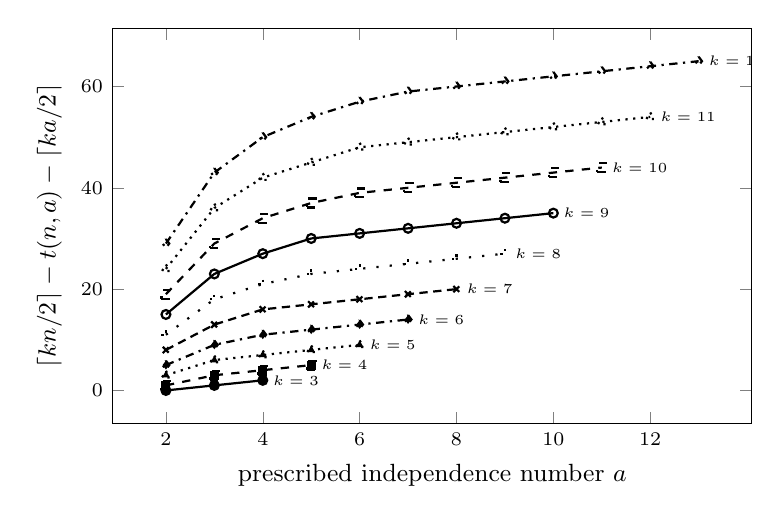
\begin{tikzpicture}
\begin{axis}[width=0.8\textwidth,height=6.6cm,xlabel={prescribed independence number $a$},ylabel={$\lceil kn/2\rceil-t(n,a)-\lceil ka/2\rceil$},tick label style={font=\scriptsize},label style={font=\small},xtick={2,4,6,8,10,12},cycle list={{solid,mark=*},{dashed,mark=square*},{dotted,mark=triangle*},{dashdotted,mark=diamond*},{densely dashed,mark=x},{loosely dotted,mark=+},{solid,mark=o},{dashed,mark=square},{dotted,mark=triangle},{dashdotted,mark=diamond}},every axis plot/.append style={line width=0.8pt}]
\addplot+[mark size=1.6pt] coordinates {(2,0) (3,1) (4,2)} node[pos=1,anchor=west,font=\tiny] {$k=3$};
\addplot+[mark size=1.6pt] coordinates {(2,1) (3,3) (4,4) (5,5)} node[pos=1,anchor=west,font=\tiny] {$k=4$};
\addplot+[mark size=1.6pt] coordinates {(2,3) (3,6) (4,7) (5,8) (6,9)} node[pos=1,anchor=west,font=\tiny] {$k=5$};
\addplot+[mark size=1.6pt] coordinates {(2,5) (3,9) (4,11) (5,12) (6,13) (7,14)} node[pos=1,anchor=west,font=\tiny] {$k=6$};
\addplot+[mark size=1.6pt] coordinates {(2,8) (3,13) (4,16) (5,17) (6,18) (7,19) (8,20)} node[pos=1,anchor=west,font=\tiny] {$k=7$};
\addplot+[mark size=1.6pt] coordinates {(2,11) (3,18) (4,21) (5,23) (6,24) (7,25) (8,26) (9,27)} node[pos=1,anchor=west,font=\tiny] {$k=8$};
\addplot+[mark size=1.6pt] coordinates {(2,15) (3,23) (4,27) (5,30) (6,31) (7,32) (8,33) (9,34) (10,35)} node[pos=1,anchor=west,font=\tiny] {$k=9$};
\addplot+[mark size=1.6pt] coordinates {(2,19) (3,29) (4,34) (5,37) (6,39) (7,40) (8,41) (9,42) (10,43) (11,44)} node[pos=1,anchor=west,font=\tiny] {$k=10$};
\addplot+[mark size=1.6pt] coordinates {(2,24) (3,36) (4,42) (5,45) (6,48) (7,49) (8,50) (9,51) (10,52) (11,53) (12,54)} node[pos=1,anchor=west,font=\tiny] {$k=11$};
\addplot+[mark size=1.6pt] coordinates {(2,29) (3,43) (4,50) (5,54) (6,57) (7,59) (8,60) (9,61) (10,62) (11,63) (12,64) (13,65)} node[pos=1,anchor=west,font=\tiny] {$k=12$};
\end{axis}
\end{tikzpicture}

\caption{Shortfall of the second-line expression $t(n,a)+\lceil ka/2\rceil$ below the degree-sum bound $\lceil kn/2\rceil$ on the shell $n=a+k+1$, one curve per $k=3,\ldots,12$ against the prescribed independence number $a$. Every plotted value is nonnegative and zero only at $(k,a)=(3,2)$, where the second line equals $f(6,2,3)=9$; at the other 74 pairs of the grid the second line cannot hold. Each curve is labeled with its $k$ and has its own mark and line style.}
\label{fig:shortfall}
\end{figure}

\subsection{Ablation of the construction}\label{sec:res-ablation}

Table~\ref{tab:ablation} lists what each ingredient contributes by removing or altering it and stating the consequence.
Rows marked [D] follow from the proofs, and rows marked [MV] are the negative controls above.

\begin{table}[ht]
\centering\small
\begin{tabular}{p{0.28\textwidth}p{0.46\textwidth}p{0.17\textwidth}}
\toprule
Ingredient removed or altered & Consequence & Evidence\\
\midrule
Complement matching in the generic residual graph & Vertices of $M$ keep residual degree $g$, so their total degree is $g+a-1=k-1<k$, and the graph cannot be $k$-connected & [D], Lemma~\ref{lem:lift}\\
Two vertices of $S$ miss the same $t\in M$ (same $H$) & $t$ has total degree $g+a-1=k-1<k$, so $G$ is not $k$-connected; the bound of two on mixed independent sets and the two-survivor argument also fail. Non-injective misses can work with a different residual degree profile, as in Section~\ref{sec:strip} & [D], Lemma~\ref{lem:lift}\\
Antipodal matching for odd $g$ & The cycle power alone is only $2r$-connected, and two blocks of $r$ deleted vertices disconnect it, so the residual graph is not $g$-connected & [D], Lemma~\ref{lem:harary}\\
One edge deleted at a vertex of degree $k$ & The connectivity falls from $k$ to $k-1$ in all 75 constructions & [MV], Table~\ref{tab:damaged}\\
Star residual graph at $a=k-1$ & The independent set of the $k$ leaves has size $k$, not $k-1$; all 6 stars fail & [MV], Section~\ref{sec:res-trees}\\
Disconnected residual graph at $a=k-1$ & No lift is $k$-connected; 10 and 285 residual graphs for $k=4,5$ fail & [MV], Table~\ref{tab:residual}\\
A triangle or a $4$-cycle in the cycle union at $a=2$ & Independence number three, or a cut of size $k-1$ & [MV], Table~\ref{tab:controls}\\
\bottomrule
\end{tabular}
\caption{Ablation of the shell construction: each row removes or alters one ingredient and states the consequence and where it is established. The first three rows are consequences of the proofs of Lemmas~\ref{lem:lift} and~\ref{lem:harary}; the last four are exact negative controls recorded in the certificates.}
\label{tab:ablation}
\end{table}

The first three rows are not exhaustive tests of every alternative construction, which could still succeed by a different route; they show that, within the proofs, each ingredient is used.
The last four rows are the converse: the properties the theorems assert are lost, as predicted, when the structure is altered, and the loss is detected by both connectivity tests and by both independence computations.
The damaged-edge row is the strictest, because it removes a single edge from a graph that has no spare edge: the constructions have exactly the degree-sum number of edges and at most one vertex of degree $k+1$, so every edge has an endpoint of degree $k$ and its deletion leaves a vertex of degree $k-1$, and every edge is needed [D, from the degree pattern].
The computation confirms the consequence for one edge in each of the 75 graphs, the first edge at the first vertex of degree $k$.

\subsection{Independent recomputation and digests}\label{sec:res-audit}

The recomputation with NetworkX \cite{NetworkX} reproduces the sizes, the connectivities and the independence numbers of all \NGraphs\ graphs, the \NHarary\ pairs of residual connectivities, the \NDamaged\ damaged-graph connectivities and the \NCycleControls\ cycle controls without a disagreement; it did not import either checker of the experiments.
Its source and the sources it checks are bound to the certificate by SHA-256 digests (Table~\ref{tab:digests}).
The script that generates the tables of this paper recomputes each digest from the file it names and stops on a mismatch.
The recomputation's summary reports \NGraphs\ graphs, \NHarary\ Harary bases, \NOdd\ cases with an odd degree sum, \NDamaged\ damaged-edge controls and \NCycleControls\ cycle controls, the same counts as the first implementation's summary, and for every one of the \NHarary\ Harary rows the connectivity of the starting graph equals $g=k-a$ exactly.
A mismatch between the two implementations on any graph would have stopped the recomputation, since each comparison is an assertion, so the agreement reported here is complete and not a sample.
Both summaries bind the proof, the certificate and the sources of the verifiers by digest, which fixes the files that the reported numbers describe.

\begin{table}[ht]
\centering\scriptsize
\setlength{\tabcolsep}{3pt}
\begin{tabular}{p{0.40\textwidth}p{0.55\textwidth}}
\toprule
File (where the digest is recorded) & SHA-256\\
\midrule
EXP-001 run.py (recorded in its certificate) & \texttt{61a3bfbedfd8b6d1f022b8338a2cc569}\newline\texttt{f23147be9f26d5e1a73015bd1b49d67a}\\
EXP-001-tree-strip/run.py (recorded in the EXP-002 certificate) & \texttt{61a3bfbedfd8b6d1f022b8338a2cc569}\newline\texttt{f23147be9f26d5e1a73015bd1b49d67a}\\
EXP-002-next-shell/run.py (recorded in the EXP-002 certificate) & \texttt{ae4d26efef9eabf23aef95dcdc56c235}\newline\texttt{b5e160510ef9729253c753a9d88af797}\\
EXP-001 certificate, line endings normalised (in the EXP-002 certificate) & \texttt{c2cb5c7322c31d4faafed2fdab221c41}\newline\texttt{13c8b3d6bc53ee5f733eff33b6d5b046}\\
EXP-002 audit.py (recorded in the recomputation output) & \texttt{f0b2e5f6cd2d7123aba5b8a8565f1f76}\newline\texttt{2515ac539706e023f85742e2afd22a9b}\\
EXP-002 proof.md (recorded in the recomputation output) & \texttt{fb63d0c2bf107e12946e53e8a394a206}\newline\texttt{c8e5a474f40d9c2273e20bdbde138d7a}\\
EXP-002 certificate (recorded in the recomputation output) & \texttt{471e311c25f636ce85a5e0961127de73}\newline\texttt{9b33c1414179fb549d81959749b8044d}\\
\bottomrule
\end{tabular}
\caption{The SHA-256 digests quoted by the saved certificates and by the independent recomputation. The table is generated by the script that also recomputes each digest from the file it names, with line endings normalised, and stops when one differs; all digests agree with the files.}
\label{tab:digests}
\end{table}

